\chapter[Theory]{Theory of trapped particles and \AE{}}
\label{chap: chapter 2}
Here, we set up the equations describing the central concepts that enter into the calculation of \AE{}.\footnote{This chapter highlights the central concepts given in references \cite{helander2005collisional,helander2014theory,helander2017available,helander2020available}.} The difficulty will be finding some way to parameterise the set given in Eq. \eqref{eq:set-of-all-distribution-functions}, especially if additional conserved quantities $\boldsymbol{y}$ are present. Using Liouville's theorem, we shall, however, be able to implicitly construct this set. More pressingly, however, is the choice of invariants considered, which we shall investigate first.


\section{Lagrangian mechanics and trapped particle orbits}
\label{sec: lagrangian mechanics and trapped particles}
As hinted at in the previous sections, trapped particles play a central role in the current thesis, and thus we highlight some important concepts required when investigating such particles. As it turns out, Lagrangian mechanics is the natural mathematical language for investigating such particles, and as such, we first start with a brief primer on these methods.
\subsection{Lagrangian mechanics}
In 1788, Joseph-Louis Lagrange, a French mathematician, wrote an elegant reformulation of Newtonian mechanics during his stay in Berlin \cite{lagrange1853mecanique}. The main benefit of the formalism carrying his name is that it is coordinate-independent, and it makes recognising certain conserved quantities trivial. The central concept in the formalism is the action, $\mathcal{S}$, which is the path integral of the Lagrangian $\mathcal{L}$,
\begin{equation}
    \mathcal{S} = \int \mathcal{L}(\boldsymbol{q}(t),\dot{\boldsymbol{q}}(t),t) \mathrm{d} t.
\end{equation}
Here, $\boldsymbol{q}$ and $\dot{\boldsymbol{q}}$ denote some arbitrary coordinate system and temporal derivatives thereof, and the Lagrangian is defined as the difference of the kinetic and potential energies, $\mathcal{L} = E_{\rm kinetic} - E_{\rm potential}$. We now seek to find a path $\boldsymbol{q}(t),\dot{\boldsymbol{q}}(t)$ that minimises the action, which may be found by introducing the addition of small variation $ \delta \boldsymbol{q}(t),\delta \dot{\boldsymbol{q}}(t)$ and imposing that the variation $\delta \mathcal{S}$ vanishes. This results in the Euler-Lagrange equation,
\begin{equation}
    \frac{\mathrm{d}}{\mathrm{d} t} \left( \frac{\partial \mathcal{L}}{\partial \dot{\boldsymbol{q}}} \right) = \frac{\partial \mathcal{L}}{ \partial \boldsymbol{q} }.
    \label{eq: EL equation}
\end{equation}
The above equation is exactly equivalent to Newton's equations of motion, but with the coordinate-system $\boldsymbol{q}$ chosen arbitrarily. If one furthermore finds that the Lagrangian depends only on $\dot{q}_i$ and \textbf{not} on $q_i$ we find that $\partial_{\dot{q}_{i}} \mathcal{L}$ is a conserved quantity. \par 
Herein lies the power of Lagrangian mechanics: find a well-chosen coordinate system $\boldsymbol{q}$, and one may readily derive constants of motion. In the next section, we specialise in the dynamics of charged particles, where we will encounter several such constants of motion. These will prove crucial when investigating \AE{}, and as such, let us carefully derive them.
\subsection{Charged particle dynamics and the first invariant}
To this end, let us first consider the Lagrangian of a (non-relativistic) particle in a magnetic field, which is given by \cite[Sec.~16]{landau2013classical}
\begin{equation}
    \mathcal{L} = \frac{1}{2} m v^2 + q\boldsymbol{A} \cdot \dot{\boldsymbol{r}},
\end{equation}
where $\boldsymbol{A}$ is the magnetic potential which satisfies $\nabla \times \boldsymbol{A} = \boldsymbol{B}$, and $q$ denotes the particle charge. One can expand this Lagrangian around the smallness of the gyroradius $\rho$ (more precisely, $\rho$ should be small compared with variations of the magnetic field), giving rise to the gyroaveraged Lagrangian. More specifically, the position vector $\boldsymbol{r}$ is split into a guiding centre and a gyrating component
\begin{equation}
    \boldsymbol{r} = \underbrace{\boldsymbol{R}}_{\text{guiding centre}} + \underbrace{\boldsymbol{\rho}}_{\text{gyration}},
\end{equation}
and takes $\boldsymbol{\rho}$ to be small. There are many accounts available of this expansion \cite{littlejohn1983variational,helander2005collisional,cary2009hamiltonian,rodriguez2022quasisymmetry}, and we refer to these references for detailed derivations. I shall simply state the result of this expansion, namely
\begin{equation}
    \overline{\mathcal{L}} \approx \frac{m}{2B}\left( \boldsymbol{B} \cdot \dot{\boldsymbol{R}} \right)^2 + q \boldsymbol{A} \cdot \dot{\boldsymbol{R}} + \frac{m(\rho \dot{\vartheta})^2}{2} + \frac{q \rho^2 \dot{\vartheta} B}{2}
\end{equation}
where $\vartheta$ is the angle of gyration. We first derive the Euler-Lagrange equation for $\dot{\vartheta}$, resulting in our first constant of motion (to the order of the expansion)
\begin{equation}
    \frac{\mathrm{d}}{\mathrm{d} t} \left( \frac{\partial \mathcal{L}}{\partial \dot{\vartheta}} \right) = \frac{\mathrm{d}}{\mathrm{d} t} \left( m \rho^2 \dot{\vartheta} + \frac{q B \rho^2}{2} \right) = 0.
    \label{eq: mu-cons general}
\end{equation}
To get this in a more familiar form, let us next investigate the Euler-Lagrange equation for $\rho$, resulting in
\begin{equation}
    \partial_\rho \overline{\mathcal{L}} = m \rho \dot{\vartheta}^2 + q \rho \dot{\vartheta} B = 0 \implies \dot{\vartheta} = -\frac{qB}{m} \equiv \Omega.
\end{equation}
Combining this with Eq. \eqref{eq: mu-cons general} we find that $\rho^2 \Omega$ is a conserved quantity. Finally realising that $\rho \Omega$ is simply the velocity perpendicular to the field line $v_\perp$, we find our desired constant of motion.
\begin{equation}
    \mu = \frac{m v_\perp^2}{2B}.
\end{equation}
Given an adequately magnetised plasma (i.e. $\rho$ should be small enough), $\mu$ is thus a conserved quantity. This will be one of the invariants that will be considered in the calculation of \AE{}. \par 
A crucial step in this derivation was finding a convenient coordinate system to express the Lagrangian in, which is where the guiding centre decomposition of the coordinate $\boldsymbol{r}$ entered. If we express $\boldsymbol{R}$ in terms of a convenient coordinate system once more, we shall find an additional constant of motion for trapped particles. The existence of such trapped particles can be readily seen as follows; first consider a point particle of mass $m$ attached to a rigid wire whose height is described by $h(x)$, in a gravitational field with constant acceleration $g$. The total energy may thus be written as the sum of the kinetic and potential components,
\begin{equation}
    E = \frac{1}{2}mv^2 + mgh(x).
\end{equation}
Compare this with the total energy of a particle in a magnetised plasma,
\begin{equation}
    E = \frac{1}{2}mv_\parallel^2 + \frac{1}{2}mv_\perp^2 = \frac{1}{2}mv_\parallel^2 + \mu B.
\end{equation}
Seeing the correspondence between the two energies, one sees that $\mu B$ can be interpreted as an effective ``potential.'' In fact, if we write down a Lagrangian with this potential, $\mathcal{L} = mv_\parallel^2/2 - \mu B$, the Euler-Lagrange equation for the parallel coordinate becomes
\begin{equation}
    m \dot{v}_\parallel = - \mu \nabla_\parallel B,
\end{equation}
and we have derived the so-called ``mirror force.'' This mirror reflects particles as they try to enter regions of stronger magnetic field. The point where the mirror force changes the sign of $v_\parallel$ is called the ``bounce point'', which, from energy considerations, must satisfy $E = \mu B$. Of further interest is the perpendicular dynamics of these trapped particles, and these dynamics are readily derived in Clebsch coordinates; the focus of the next section.

\subsection{A brief intermezzo on Clebsch coordinates}
The convenient choice of coordinates turns out to be the so-called Clebsch coordinates, which we briefly review here (one may refer to \citet{d2012flux} for a more complete overview, and this section follows Ref. \cite{helander2014theory}). Assuming that one satisfies magnetohydrodynamic equilibrium conditions, $\boldsymbol{J} \times \boldsymbol{B} = \nabla  p$ (with $\boldsymbol{J}$ being the current density), the magnetic field in toroidal geometry may be written as
\begin{equation}
    \boldsymbol{B} = B_1(p,\theta,\phi) \nabla p \times \nabla \theta + B_2(p,\theta,\phi) \nabla \phi \times \nabla p.
\end{equation}
Here, $\theta$ and $\phi$ are arbitrary angles that parameterise a surface of the torus, $p$ is the pressure, and $B_1$ and $B_2$ are functions we wish to find. In this form, we have ensured that $\boldsymbol{B} \cdot \nabla p = 0$, as required by the equilibrium conditions. We furthermore require that the magnetic field be divergence-free, i.e. $\nabla \cdot \boldsymbol{B} = 0$, which results in 
\begin{equation}
    \left( \frac{\partial B_1}{\partial \phi} + \frac{\partial B_2}{\partial \theta} \right) \nabla p \cdot \left( \nabla \theta \times \nabla \phi \right) = 0 \implies \frac{\partial B_1}{\partial \phi} + \frac{\partial B_2}{\partial \theta} = 0.
\end{equation}
As such, $B_1$ and $B_2$ can in general be represented as 
\begin{subequations}
\begin{alignat}{4}
B_1 &= \partial_\theta f + g(p), \\
B_2 &= \partial_\phi f   + h(p).
\end{alignat}
\end{subequations}
for some functions $f(p,\theta,\phi)$, $g(p)$, and $h(p)$. If we now conveniently choose
\begin{subequations}
\begin{alignat}{4}
B_1 &= \psi'(p) \left( 1 + \partial_\theta \lambda \right), \\
B_2 &= \chi'(p) - \psi'(p) \partial_\phi \lambda,
\end{alignat}
\end{subequations}
the magnetic field may be expressed in its familiar form
\begin{equation}
    \boldsymbol{B} = \nabla \psi \times \nabla \theta + \nabla \phi \times \nabla \chi,
\end{equation}
where one can show that $2\pi\psi$ and $2\pi\chi$ correspond to the toroidal and poloidal fluxes of the device, respectively \cite{helander2014theory}. These fluxes are in turn related to the rotational transform, via
\begin{equation}
    \frac{\boldsymbol{B} \cdot \nabla \theta}{\boldsymbol{B} \cdot \nabla \phi}=\frac{\mathrm{d} \chi }{\mathrm{d} \psi} = \iota,
\end{equation}
and hence the magnetic field may be simplified to
\begin{equation}
    \boldsymbol{B} = \nabla \psi \times \nabla \left( \theta - \iota \phi \right) \equiv \nabla \psi \times \nabla \alpha.
    \label{eq: clebsch-representation}
\end{equation}
Eq. \eqref{eq: clebsch-representation} is the \textit{Clebsch representation} of the magnetic field, where $\psi$ is often called the radial coordinate, and $\alpha$ is called the binormal coordinate. Since $\boldsymbol{B} \cdot \nabla \alpha = 0$, $\alpha$ is constant along the magnetic field, as is $\psi$. As such we require a final coordinate parameterising the path along the magnetic field line, for which we choose the arc length $\ell$, which is unique up to an offset. The three coordinates $(\psi,\alpha,\ell)$ will be called Clebsch coordinates henceforth, and they are a natural coordinate system to describe quantities local to a magnetic field line. Finally, one may readily verify that valid magnetic potentials corresponding to the Clebsch representation are $\boldsymbol{A} = -\alpha \nabla \psi$ and $\boldsymbol{A} = \psi \nabla \alpha$. \par 
\subsection{The second invariant}
With our understanding of Clebsch coordinates on solid ground, let us investigate the gyro-averaged Lagrangian once more, focussing on the dynamics encoded in $\boldsymbol{R}$. As such, let us drop terms that do not explicitly involve the guiding centre, giving 
\begin{equation}
    \overline{\mathcal{L}} \approx \frac{m}{2} (\boldsymbol{b} \cdot \dot{\boldsymbol{R}})^2 + q \boldsymbol{A} \cdot \dot{\boldsymbol{R}} - \mu B,
\end{equation}
where we have defined $\boldsymbol{b} = \boldsymbol{B}/B$. Set $\boldsymbol{A} = \psi \nabla \alpha$, so that $\boldsymbol{A} \cdot \dot{\boldsymbol{R}} = \psi \dot{\alpha}$, which can be verified by employing the identity $\dot{\boldsymbol{R}}=\dot{\psi} \partial_\psi \boldsymbol{R} + \dot{\alpha} \partial_\alpha \boldsymbol{R} +\dot{\ell} \partial_\ell \boldsymbol{R}$. Next, investigate the Euler-Lagrange equation for $\alpha$. Focussing on the left-hand side of Eq. \eqref{eq: EL equation}, we find the following
\begin{equation}
\begin{aligned}
    \frac{\partial \mathcal{L}}{\partial \dot{\alpha}} &= m (\boldsymbol{b} \cdot \dot{\boldsymbol{R}}) (\boldsymbol{b} \cdot \partial_{\dot{\alpha}} \dot{\boldsymbol{R}}) + q \psi \\
    &= m v_\parallel \boldsymbol{b} \cdot \boldsymbol{R} + q \psi,
\end{aligned}
\end{equation}
where the parallel velocity is defined as $v_\parallel = \boldsymbol{b} \cdot \dot{\boldsymbol{R}}$. Now, we turn our attention to the right-hand side of Eq. \eqref{eq: EL equation}, and we find
\begin{equation}
    \frac{\partial \mathcal{L}}{\partial \alpha} = - \mu \partial_\alpha B.
\end{equation}
All in all, the Euler-Lagrange equation thus becomes
\begin{equation}
    \frac{\mathrm{d}}{\mathrm{d}t}\left( \psi + \frac{m v_\parallel }{q} \boldsymbol{b} \cdot \partial_\alpha \boldsymbol{R} \right) = - \frac{\mu}{q} \partial_\alpha B,
    \label{eq: euler-lagrange for psi}
\end{equation}
Recognise that the right-hand side of the above equation may be rewritten via energy conservation,
\begin{equation}
    E = \frac{m v_\parallel^2}{2} + \mu B.
\end{equation}
We integrate the above equation with respect to time, across one bounce-motion of a trapped particle. Realising that the term involving $v_\parallel$ vanishes at the bounce-points, the integral may be written as\footnote{We note here that one can also integrate across the entire domain for passing particles, and analogous arguments can be made to show that passing particles conserve a passing equivalent of $\mathcal{J}$. This will be elaborated on further in the thesis.}
\begin{equation}
    \int_{\rm bounce} \frac{\mathrm{d}\psi}{\mathrm{d}t} \mathrm{d}t = \frac{1}{q} \int_{\rm bounce} m v_\parallel  \partial_\alpha v_\parallel \mathrm{d}t.
    \label{eq: euler-lagrange for psi}
\end{equation}
If we denote that total excursion in $\psi$ after a full bounce-motion as $\Delta \psi$, and we furthermore recognise that we may approximate $\mathrm{d}t = \mathrm{d} \ell/v_\parallel$, we find our central result
\begin{equation}
    \left( \frac{\partial \mathcal{J}}{\partial \alpha} \right)_{\psi,\mu,E} = + q \Delta\psi,
    \label{eq: dJdalpha}
\end{equation}
where we have introduced the second adiabatic invariant $\mathcal{J} = \int_{\rm bounce} m v_\parallel \mathrm{d}\ell$. The Euler-Lagrange equation for $\psi$ following the exact same steps results in
\begin{equation}
    \left( \frac{\partial \mathcal{J}}{\partial \psi} \right)_{\alpha,\mu,E} = - q \Delta\alpha.
    \label{eq: dJdpsi}
\end{equation}
As a final step, let us investigate how the second adiabatic invariant changes along an orbit. Calculating the total differential,
\begin{equation}
    \Delta \mathcal{J} = \frac{\partial \mathcal{J}}{\partial \psi} \Delta \psi + \frac{\partial \mathcal{J}}{\partial \alpha} \Delta \alpha = 0,
    \label{eq: cons of j}
\end{equation}
and we have thus proven invariance of $\mathcal{J}$. The structure of Eq. \eqref{eq: cons of j} is furthermore indicative of the fact that $\mathcal{J}$ acts as a Hamiltonian for trapped particles, which can be made rigorous by taking an appropriate bounce average of the Lagrangian. \par 
As a final step, let us make some observations that will allow us to relate $\mathcal{J}$ to typical trapped particle quantities. Firstly, we express the second adiabatic invariant through energy conservation as $\mathcal{J} = \int \sqrt{2m} \sqrt{E - \mu B} \mathrm{d} \ell$. If we take the partial of this expression with respect to $E$, one finds the following,
\begin{equation}
    \left(\frac{\partial \mathcal{J}}{\partial E}\right)_{\psi,\alpha,\mu} = \int_{\rm bounce} \sqrt{\frac{m}{2}} \frac{\mathrm{d}\ell}{\sqrt{E - \mu B}} = \int_{\rm bounce} \frac{\mathrm{d} \ell}{v_\parallel} \equiv \tau_b.
\end{equation}
Therefore, we find that $\partial_E \mathcal{J}$ simplifies to the total time it takes to complete one complete bounce motion, $\tau_b$. As such, we may calculate the velocities in the $\psi$ and $\alpha$ directions by using 
\begin{subequations}
\begin{alignat}{4}
\omega_\psi &\equiv \frac{\Delta \psi}{\tau_b} = &\frac{1}{q} \frac{\left( \partial_\alpha \mathcal{J} \right)_{\psi,\mu,E}}{\left(\partial_E \mathcal{J}\right)_{\psi,\alpha,\mu}}, \\
\omega_\alpha &\equiv \frac{\Delta \alpha}{\tau_b} = - &\frac{1}{q} \frac{\left( \partial_\psi \mathcal{J} \right)_{\alpha,\mu,E}}{\left(\partial_E \mathcal{J}\right)_{\psi,\alpha,\mu}}. \label{eq: omega_alpha}
\end{alignat}
\end{subequations}
The above two equations give us the bounce-averaged velocity of particles in the radial ($\psi$) and binormal ($\alpha$) direction. Such bounce-averaged drifts, as they are colloquially called, play a central role in many areas of magnetic-confinement fusion research.
\subsection{The physical relevance of $\mathcal{J}$}
With our knowledge of the second adiabatic invariant and its relation to drifts in mind, let us now investigate how these drifts relate to the fundamental concepts of stellarator physics. Both drifts play important roles in somewhat disjoint fields, with the radial drift being closely connected to neoclassical transport and the binormal and radial drifts playing an important role in the gyrokinetic stability of certain modes. First, we investigate the radial drift.  \par 
As hinted at in the introduction, the stellarator community has long focused on understanding and minimising neoclassical transport, which is intimately linked with $\omega_\psi$, the bounce-averaged radial drift. A simple physical picture to keep in mind is that, if $\omega_\psi \neq 0$, trapped particles will drift across flux surfaces, until they eventually reach the wall of the torus. Therefore, a minimal condition for the confinement of particles is that $\omega_\psi$ should be zero, and magnetic fields that satisfy this condition are called \textit{omnigeneous} \cite{catto1981omnigenous}. It is under the broad concept of omnigeneity that we find many foundational concepts of stellarator physics, such as quasi-symmetry \cite{boozer1983transport,landreman2012omnigenity,landreman2022magnetic,rodriguez2020necessary,rodriguez2022quasisymmetry} and quasi-isodynamicity \cite{nuhrenberg2010development,goodman2022constructing}. Tokamaks are, as a consequence of their axisymmetry, exactly omnigenous. \par 
The bounce-averaged binormal drift $\omega_\alpha$ on the other hand, plays a central role in determining gyrokinetic (in)stability of trapped particles in omnigenous systems \cite{rosenbluth1971finite,proll2012resilience,helander2013collisionless}, where magnetic fields with the so-called maximum-$\mathcal{J}$ property have stability. Such devices are signified by a monotonically decreasing $\mathcal{J}$ as a function of $\psi$, implying that $\omega_\alpha \propto \partial_\psi \mathcal{J}$ is of one sign. Although the stability of such devices is ultimately the consequence of a resonance condition between trapped particle drifts and a diamagnetic drift wave driven by a density gradient, it can be understood in simpler terms, as noted by \citet{helander2012stellarator}. Suppose there is some instability in an omnigenous device which perturbs the energy of a particle, but does not break the invariance of $\mathcal{J}$. Then we have
\begin{equation}
    \mathrm{d} \mathcal{J} = \partial_E \mathcal{J} \mathrm{d}E + \partial_\psi \mathcal{J} \mathrm{d}\psi =0 \implies \Delta E = - \frac{\partial_\psi \mathcal{J}}{\partial_E \mathcal{J}} \Delta \psi
\end{equation}
The particle takes/dumps some energy $\Delta E$ from/into the instability depending on the sign of $\partial_\psi \mathcal{J}$. More precisely, the particle \textit{loses} energy to the instability, thereby enhancing in, by moving radially outwards if $\partial_\psi \mathcal{J} > 0$. Conversely, the particle \textit{takes} energy from the instability by moving radially outwards if $\partial_\psi \mathcal{J} < 0$. Therefore, an outward particle flux tends to take energy from the instability if $\partial_\psi \mathcal{J} < 0$, thus stabilising the instability. Geometries with $\partial_\psi \mathcal{J} < 0$ are thus favourable, and we have shown the beneficial nature of maximum-$\mathcal{J}$ devices. \par 
Finally, it is worth considering to what extent the adiabatic invariance of $\mu$ and $\mathcal{J}$ is met under realistic circumstances, present in fusion reactors. To this end, we consider some typical frequencies found in such reactors for the cyclotron motion, the bounce motion, and the turbulence. Denote the gyrofrequency of some species $s$ by $\Omega_s = Ze B / m_s$. To estimate the bounce time, we set $\tau_{b,s} = L/v_\parallel=\iota R_0/\sqrt{T/m_s}$, where we have taken the length scale to be the connection length, which relates to the major radius $R_0$ and $\iota$ through $L\sim R_0/\iota$. Furthermore, we have approximated the parallel velocity by the thermal velocity, resulting in the bounce frequency being $\omega_{b,s}\sim \iota \sqrt{T}/R_0\sqrt{m_s}$. Finally, the typical turbulence frequencies actually depend on the turbulence type considered. We shall focus on turbulence types that take place on the ion-gyroradius scale, such as the ion-temperature gradient (ITG) mode or the trapped electron mode (TEM) \cite{helander2013collisionless,plunk2014collisionless}, and note that the current ordering may be broken if one instead considers, e.g. electron-temperature gradient modes \cite{lee1987collisionless}. ITG and TEM have frequencies on the order of the diamagnetic drift (see \citet{de2012guiding} for expressions of this pressure gradient driven drift), which we estimate as $v_D \sim p \nabla \ln(p)/ZenB \sim p \omega_p/ZaenB$, with $a$ being the minor radius of the device and $\omega_p = a\nabla \ln p$ being the normalised pressure gradient. The frequency can now be found as $\omega_D \sim v_D/a \sim p \omega_p /Za^2 e n B$. All in all, considering hydrogen ions and electrons as our species, we find that the frequencies compare as
\begin{equation*}
    \begin{aligned}
        &\Omega_e & \colon & \Omega_i & \colon & \omega_{b,e} & \colon & \omega_{b,i} & \colon & \omega_{D} & \\
        & \frac{eB}{m_e} & \colon & \frac{eB}{m_i} & \colon & \frac{\iota}{R_0}\sqrt{\frac{T}{m_e}} & \colon & \frac{\iota}{R_0} \sqrt{\frac{T}{m_i}} & \colon & \frac{p \omega_p}{a^2 enB}  & \\
        & \frac{m_i}{m_e} & \colon & 1 & \colon & \epsilon \iota \rho_i^* \sqrt{\frac{m_i}{m_e}} & \colon & \epsilon \iota \rho_i^* & \colon &  (\rho_i^*)^2 \omega_p &.
    \end{aligned}
\end{equation*}
Here we have defined the ion gyroradius as $\rho_i \equiv \sqrt{m_i T}/eB$ and its dimensionless equivalent $\rho_i^*\equiv \rho_i/a$. In addition, we have introduced the inverse aspect ratio $\epsilon \equiv a/R_0$. Now $m_i/m_e$ is on the order of a thousand, $\rho_i^*$ is typically a couple percent, we take $\epsilon \iota \sim 10 \%$, and the logarithmic gradient is typically $\omega_p \gtrapprox 1$. We now have our final ordering
\begin{equation}
    \Omega_e  \gg \Omega_i \gg \omega_{b,e} \gg \omega_{b,i} \sim \omega_{D}.
\end{equation}
Therefore, we find that for electrons, $\mu$ and $\mathcal{J}$ are typically conserved. On the other hand, ions have bounce frequencies too close to characteristic frequencies of the turbulence, and as such invariance of $\mathcal{J}$ is expected to be broken. Therefore, a theory of \AE{} that takes $\mu$ and $\mathcal{J}$ as invariants should be interpreted to be valid only for electrons in fusion devices.\footnote{Some care should be taken here. Formally, particles that approach a (local) maximum in $B$ along a field line have divergent bounce times, analogous to a simple pendulum at large amplitudes \cite{lewowski2002period}. This subset of particles breaks the invariance of $\mathcal{J}$, as their frequencies approach zero. Furthermore, both the turbulence and the thermal velocity have a distribution of frequencies, and the tails of these distributions may break the orderings presented. We ignore such complications here.} \par
Both omnigeneity and the maximum-$\mathcal{J}$ property will be shown to be intimately related to the \AE{} of trapped particles. More precisely, it will be shown that the \AE{} vanishes \textit{exactly} in magnetic fields which satisfy both conditions and returns a nonzero value as one deviates from it. It thus provides a physical measure (it is an energy after all) to assess how close a geometry is to being both omnigenous and maximum-$\mathcal{J}$. Before delving into such details, though, we should strengthen our understanding of \AE{} and how it depends on chosen invariants, which we will do in the next sections.



\section{On Liouville, invariants, and ground states}
Let us start by parameterising the phase-space $\boldsymbol{x}$ in terms of the coordinates $\boldsymbol{x}=(\boldsymbol{y},\boldsymbol{z})$, where $\boldsymbol{z}$ are the remaining coordinates describing the phase-space. This parameterisation furthermore has the Jacobian $\sqrt{g}$, and the Vlasov equation for the particle distribution function becomes
\begin{equation}
    \frac{\partial (f\sqrt{g})}{\partial t} + \dot{\boldsymbol{z}} \cdot  \nabla_{\boldsymbol{z}} (f\sqrt{g}) = 0,
    \label{eq: continuity equation in general}
\end{equation}
where all terms with $\dot{\boldsymbol{y}}=0$ due to the constancy of $\boldsymbol{y}$. We next realise that since the phase-space volume is conserved as a consequence of Liouville's theorem, there is an additional equation that describes the dynamics of $\sqrt{g}$. Noting that $V = \int \sqrt{g} \mathrm{d}\boldsymbol{x}$ and incompressibility imply $\mathrm{d}V/\mathrm{d}t=0$, one finds
\begin{equation}
    \frac{\partial \sqrt{g}}{\partial t} + \dot{\boldsymbol{z}} \cdot \nabla_{\boldsymbol{z}} \sqrt{g} = 0.
    \label{eq: Liouville theorem for Jacobian}
\end{equation}
Combining Eqs. \eqref{eq: continuity equation in general} and \eqref{eq: Liouville theorem for Jacobian}, we find the following equation describing the dynamics of the distribution function,
\begin{equation}
    \sqrt{g} \left( \frac{\partial f}{\partial t} + \dot{\boldsymbol{z}} \cdot \nabla_{\boldsymbol{z}} f \right) = 0.
\end{equation}
If we now multiply the above equation by some function $G'[f]$, use the chain rule, and finally integrate over $\boldsymbol{z}$, one finds
\begin{equation}
    \frac{\mathrm{d}}{\mathrm{d} t} \int G[f] \sqrt{g} \: \mathrm{d} \boldsymbol{z} = 0 \implies \int G[f] \sqrt{g} \: \mathrm{d} \boldsymbol{z} = \mathrm{const.}
    \label{eq: constraints G[f]}
\end{equation}
Eq. \eqref{eq: constraints G[f]} puts an uncountably infinite number of constraints on $f$, as we may choose any well-behaved function $G[f]$.\footnote{These constraints are often called Casimir invariants \cite{ye1992action}, named after Hendrick Casimir. A bit of trivia, Casimir had spent quite some time in Eindhoven (home of the current thesis), where he first postulated the existence of the Casimir effect. This attractive force between conducting plates was subsequently measured in Philips' NatLab \cite{lambrecht2002casimir,sarlemijn2012physics}.} In essence, this equation describes Liouville's theorem from the perspective of the distribution function: since phase-space flow is incompressible, the set of accessible functions is heavily constrained. To gain more insight, let us parameterize the functions $G[f]$ as follows,
\begin{equation}
    G[f] = H[f-\phi]; \quad \forall \phi \in \mathbb{R}
    \label{eq: casimir inv.}
\end{equation}
where $\phi$ is some scalar constant and $H[x]$ is the Heaviside function of $x$. We then see that the set $\mathcal{F}_L$ consists of all the distribution functions satisfying
\begin{equation}
    \int H[f - \phi]  \sqrt{g} \: \mathrm{d} \boldsymbol{z} = \int H[f_i(\boldsymbol{y},\boldsymbol{z})-\phi] \sqrt{g} \: \mathrm{d} \boldsymbol{z} \iff f \in \mathcal{F}_L[f_i;\boldsymbol{y}],
    \label{eq:restricted parameter space}
\end{equation}
for all $\phi \in \mathbb{R}$. Here $f_i\equiv f(t=0,\boldsymbol{x})$ is the initial condition/distribution function, which determines the set of accessible distribution functions. Summarising, we find that, if there is a continuity equation for $f$ with a Liouville theorem, $f \in \mathcal{F}_L[f_i;\boldsymbol{y}]$ where $f_i$ is the initial condition. \par 
With the above framework ready, we can now derive crucial properties of the ground state. We remind ourselves that we wish to find the distribution function in $\mathcal{F}_L[f_i;\boldsymbol{y}]$ that minimises
\begin{equation}
    E_T[f] = \int \epsilon f \sqrt{g} \: \mathrm{d} \boldsymbol{x}.
\end{equation}
We realise that since $\mathcal{F}_L$ is independent at different values of $\boldsymbol{y}$, the minimisation problem can be solved on sheaths of constant $\boldsymbol{y}$. In other words, we may instead minimise
\begin{equation}
    E_T[f;\boldsymbol{y}]= \int \epsilon(\boldsymbol{y},\boldsymbol{z}) f \sqrt{g} \: \mathrm{d}\boldsymbol{z},
\end{equation}
for each $\boldsymbol{y}$ to find the state that minimises the thermal energy. To enforce that $f$ obeys Eq. \eqref{eq:restricted parameter space}, we use a Lagrange multiplier $\lambda(\phi,\boldsymbol{y})$ to construct a functional $W$ that will be minimised. Let us thus define
\begin{equation}
    W[f,\lambda] \equiv E_T[f;\boldsymbol{y}] - \int \lambda\mathrm{d} \phi \left( \int \left\{ H[f - \phi]- H[f_i - \phi] \right\}\sqrt{g}  \mathrm{d} \boldsymbol{z} \right),
\end{equation}
where the term involving the Lagrange multiplier ensures that the factor in brackets vanishes for all $\phi$, i.e. Eq. \eqref{eq:restricted parameter space} is satisfied. We now vary $W$ with respect to $f$ (or equivalently take the functional derivative) and find
\begin{equation*}
\begin{aligned}
    \delta W_f &\equiv W[f+ \delta f,\lambda]-W[f,\lambda] \\
    &= \int \epsilon (\delta f) \sqrt{g} \mathrm{d} \boldsymbol{z} - \int (\delta f) \lambda(\phi,\boldsymbol{y}) \delta[f - \phi] \mathrm{d} \phi \sqrt{g} \mathrm{d} \boldsymbol{z}  \\
    &= \int \epsilon (\delta f) \sqrt{g} \mathrm{d} \boldsymbol{z} - \int(\delta f) \lambda(f,\boldsymbol{y}) \sqrt{g} \mathrm{d} \boldsymbol{z} \\
    &= \int \delta f \left( \epsilon - \lambda(f,\boldsymbol{y}) \right) \sqrt{g} \mathrm{d} \boldsymbol{z}.
\end{aligned}
\end{equation*}
Here, $\delta[x]$ is the Dirac-delta distribution, and we have used its sifting property. Since we are at a minimum, we require $\delta W_f=0$ for all $\delta f$, which in turn implies that the ground state must satisfy
\begin{equation}
     \lambda(f_g,\boldsymbol{y})=\epsilon \implies f_g = f_g(\epsilon,\boldsymbol{y}),
     \label{eq: ground state dependence}
\end{equation}
thus the ground state depends on the particle energy $\epsilon$ and additional conserved quantities $\boldsymbol{y}$, \textit{alone.} \par
This is a necessary, but not sufficient condition for a distribution function to be a ground state. In addition to requiring that $f_g$ be a stationary point of functional $W$, we further require that it is a \textit{minimum}. This corresponds to having
\begin{equation}
    \delta^2 W_f \equiv \delta W[f+ \delta f] - \delta W[f] > 0,
\end{equation}
and one may verify that this second variation becomes
\begin{equation}
    \delta^2 W_f = - \int (\delta f)^2 \frac{\partial \lambda}{\partial f} \sqrt{g} \: \mathrm{d} \boldsymbol{z}.
\end{equation}
Therefore, we require $\partial_f \lambda < 0$. This may be reduced further by taking the derivative of Eq. \eqref{eq: ground state dependence} with respect to $f$ at fixed $\boldsymbol{y}$, resulting in $\partial_f \lambda = \partial_f \epsilon$. We thus find that a second condition on the ground state is
\begin{equation}
     \left(\frac{\partial f_g}{\partial \epsilon} \right)_{\boldsymbol{y}} \leq 0,
\end{equation}
i.e. the ground state must be a \textit{decreasing} function in its first argument, the particle energy. \par 
It is worthwhile to take a step back and interpret the results found. It has long been known that distributions that violate $\partial_\epsilon f \leq 0$ can be unstable \cite{taylor1963some} (with the most clear example being the bump-on-tail instability \cite{drtjmmond1962non}), and one may arrive at a similar conclusion by investigating the entropy of the electric field \cite{minardi1985thermodynamics}. By investigating \AE{}, we arrive at the same conclusion, as may be understood as follows. Suppose that we start our system with an initial condition $f_i$, which has $f_i(\epsilon)$ and $\partial_\epsilon f_i \nleq 0$. We can then immediately conclude that the initial condition is not a ground state, and therefore there will be some associated $A = E[f_i] - E[f_g]>0$. On the contrary, if one were to start with a ground state, the system would be stable to begin with since $A=0$. The main benefit of \AE{} is that we may also \textit{quantify} how far from stability one is, instead of relying on binary statements. 

\subsection{Calculating the ground state and the \AE{}}
With the properties of the ground state found, we are now able to set up equations that describe the ground state and the associated \AE{}. To find the ground state, let us first investigate Eq. \eqref{eq:restricted parameter space}, where we set $f$ to be the ground state $f_g$. One finds
\begin{equation}
    \int H[f_g(\epsilon,\boldsymbol{y}) - \phi] \sqrt{g} \: \mathrm{d} \boldsymbol{z} = \int H[f_i(\boldsymbol{y},\boldsymbol{z}) - \phi] \sqrt{g} \: \mathrm{d} \boldsymbol{z}.
\end{equation}
We realise that since the ground state is monotonic in its first argument, we can define an inverse function $f^{-1}$ which satisfies $f^{-1} \circ f =\epsilon$. Noting that $f_g > \phi \implies \epsilon < f^{-1}(\phi)$ since $\partial_\epsilon f_g \leq 0$, and defining $f^{-1}(\phi)\equiv \epsilon_\phi$ as our free parameter, we arrive at the following equation that describes the ground state
\begin{equation}
    \int H[\epsilon_\phi - \epsilon(\boldsymbol{y},\boldsymbol{z})] \sqrt{g} \: \mathrm{d} \boldsymbol{z} = \int H[f_i(\boldsymbol{y},\boldsymbol{z}) - f_g(\epsilon_\phi,\boldsymbol{y})] \sqrt{g} \: \mathrm{d} \boldsymbol{z}.
    \label{eq: integral for ground state}
\end{equation}
The above equation is nonlinear integral equation, whose solution gives the ground state $f_g(\epsilon,\boldsymbol{y})$. It is often useful to instead consider the derivative of the above equation with respect to $\epsilon_\phi$, which gives
\begin{equation}
    \left( \frac{\partial f_g}{\partial \epsilon_\phi} \right)_{\boldsymbol{y}} = - \frac{\int \delta[\epsilon_\phi - \epsilon(\boldsymbol{y},\boldsymbol{z})] \sqrt{g} \: \mathrm{d} \boldsymbol{z}}{\int \delta[f_i(\boldsymbol{y},\boldsymbol{z}) - f_g(\epsilon_\phi,\boldsymbol{y})] \sqrt{g} \: \mathrm{d} \boldsymbol{z}}.
    \label{eq:integro-diff for ground state}
\end{equation}
Note that this nonlinear integro-differential equation for $f_g$ has a right-hand side which is always negative, as is required for any ground state. \par 
The solution to Eqs. \eqref{eq: integral for ground state} and \eqref{eq:integro-diff for ground state} give us the ground state, with which the calculation of \AE{} becomes trivial. To find the available energy, one simply calculates the difference in thermal energy between the initial condition and the ground state, i.e. 
\begin{equation}
    A = \int \epsilon \left( f_i - f_g \right) \sqrt{g} \: \mathrm{d}\boldsymbol{y} \mathrm{d}\boldsymbol{z}.
    \label{eq: available energy central equation}
\end{equation}
the above equation is the central figure of merit investigated in the current thesis. Let us gain some familiarity with the above equations by working out two analytically tractable examples.

\section{Example: the \AE{} of a single waterbag distribution}
The examples shown in this section are the result of a collaboration with R.J. Ewart, an expert in the closely related field of collisionless relaxation of Lynden-Bell plasmas \cite{ewart2022collisionless,ewart2023non}.\footnote{Besides Ewart's impressive work on Lynden-Bell plasmas, he is responsible for one of the more amusing analogies in the field of plasma-turbulence given in Ref. \cite{ewart2022collisionless}. Likening the Vlasov equation and its nonlinear dynamics to a block of marble, Ewart continues: "Of course, Michelangelo's David was wholly contained within a block of marble, which did not, however, provide great insight into what could lie beneath \cite{coonin2014marble}."} Ewart pointed out that an important simplifying step in the considerations of Lynden-Bell plasmas, the so-called waterbag representation, could similarly simplify calculations of the \AE{}, prompting the investigation presented in this section. \par 
In the waterbag representation, the distribution function is discretised in a manner somewhat analogous to a Lesbegue integral. That is, we restrict the initial distribution function to take on only a discrete set of values, that is, $f_i \in [0,\eta_1,\eta_2,\dots,\eta_k]$. This results in the set invariants of Eq. \eqref{eq: casimir inv.} simplifying to a discrete set. In addition, let us consider the simplest cases possible of this waterbag representation, where we set the initial distribution function equal to
\begin{equation}
f_i(\boldsymbol{r},\boldsymbol{v}) = 
\Bigg\{
    \begin{array}{lr}
        \eta, & \text{if } \epsilon < \mathcal{E}(\boldsymbol{r})\\
        0, & \text{otherwise}.
    \end{array}
\end{equation}
Such a distribution function with only one non-zero value of $\eta$ is called a single-waterbag distribution function, and it will allow us to calculate the \AE{} in two cases. Let us also note that the spatial variation of $\mathcal{E}(\boldsymbol{r})$ encodes gradients in the density, which can be seen as follows. Realise that the velocity space component of the integral is isotropic, since it only depends on $v^2$. Therefore, the velocity-space integral reduces to
\begin{equation}
    \mathrm{d}\boldsymbol{v}=4\pi v^2 \mathrm{d}v = \frac{4 \pi \sqrt{2}}{m^{3/2}} \sqrt{\epsilon} \mathrm{d} \epsilon.
\end{equation}
Now, we may perform the integral across velocity space to find the density, i.e.,
\begin{equation}
\begin{aligned}
    n(\boldsymbol{r}) &= \int f_i \mathrm{d} \boldsymbol{v} \\ 
    &= \frac{4 \pi \sqrt{2}}{m^{3/2}} \eta \int_{0}^{\mathcal{E}(\boldsymbol{r})} \sqrt{\epsilon} \mathrm{d} \epsilon \\ 
    &= \frac{8 \pi \eta \sqrt{2}}{3 m^{3/2}} \mathcal{E}(\boldsymbol{r})^{3/2}.
\end{aligned}
\end{equation}
Thus, for constant $\mathcal{E}(\boldsymbol{r})$, there are no gradients in the system. For varying $\mathcal{E}(\boldsymbol{r})$, however, there are gradients and we shall see that this results in non-zero \AE{}.

\subsection{Case I: unconstrained \AE{}}
Let us first consider the case in which no additional invariants are imposed, aside from those arising from Liouville. The integral equation for the ground state, as given in \eqref{eq: integral for ground state}, now simplifies to
\begin{equation}
    \int H \left[\epsilon_\phi - \frac{1}{2}mv^2 \right] \mathrm{d} \boldsymbol{v}\mathrm{d} \boldsymbol{r} = \int H[f_i(\boldsymbol{r},\boldsymbol{v}) - f_g(\epsilon_\phi)] \mathrm{d} \boldsymbol{v}\mathrm{d} \boldsymbol{r}.
    \label{eq: integral for ground state waterbag}
\end{equation}
Let us first realise that the velocity space component of the integral is isotropic, since it only depends on $v^2$. Therefore, the velocity-space integral reduces to $\mathrm{d}\boldsymbol{v}=4\pi v^2 \mathrm{d}v$. The integrand on the left-hand side of Eq. \eqref{eq: integral for ground state waterbag} returns one for $v^2 \in [0,2 \epsilon_\phi/m)$, and zero otherwise. All in all, the velocity-space integral on the left-hand side becomes
\begin{equation}
    4 \pi\int_0^{\sqrt{2 \epsilon_\phi/m}} v^2 \mathrm{d}v = \frac{4 \pi}{3} \left( \frac{2 \epsilon_\phi}{m} \right)^{3/2}.
\end{equation}
Similarly, we realise that the integral on the right-hand side is isotropic in velocity-space, as it also depends on $v^2$ alone. Employing completely analogous arguments (i.e., the integration range is set by $\mathcal{E}(\boldsymbol{r})$), one finds that the velocity-space integral becomes
\begin{equation}
    4 \pi \int_0^{\sqrt{2\mathcal{E}(\boldsymbol{r})/m}} v^2 \mathrm{d} v =   \frac{4 \pi}{3} \left( \frac{2 \mathcal{E}(\boldsymbol{r})}{m} \right)^{3/2}.
\end{equation}
Finally, the ground-state equation reduces to
\begin{equation}
    \epsilon_\phi = \left \langle \mathcal{E}(\boldsymbol{r})^{3/2} \right\rangle^{2/3},
    \label{eq: transition energy unconstrained}
\end{equation}
where we have defined the volume averaging operator $\langle ... \rangle = \int ... \mathrm{d} \boldsymbol{r} / \int \mathrm{d} \boldsymbol{r}$. Eq. \eqref{eq: transition energy unconstrained} gives us the energy at which the ground state $f_g$ drops from $\eta$ to zero, i.e.
\begin{equation}
f_g(\epsilon) = 
\Bigg\{
    \begin{array}{lr}
        \eta & \text{if } \epsilon < \epsilon_\phi, \\
        0 &   \text{if } \epsilon > \epsilon_\phi, 
    \end{array}
\end{equation}
and we realise that the ground state has no spatial dependence anymore: the gradients are fully flattened. Now we are in a position to evaluate \AE{}. The energy of the initial distribution function can be evaluated by computing the integral
\begin{equation}
\begin{aligned}
    E_i &= \int \epsilon f_i \mathrm{d} \boldsymbol{v}\mathrm{d} \boldsymbol{r} \\
    &= 4 \pi \frac{m\eta}{2} \int \mathrm{d} \boldsymbol{r}\int_0^{\sqrt{2\mathcal{E}(\boldsymbol{r})/m}} v^4 \mathrm{d}v \\
    &= V \frac{2 \pi}{5} m\eta \left( \frac{2}{m} \right)^{5/2} \left \langle \mathcal{E}(\boldsymbol{r})^{5/2} \right \rangle,
\end{aligned}
\end{equation}
where $V$ denotes the total real-space volume. The ground state energy can completely analogously be computed, and one finds
\begin{equation}
\begin{aligned}
    E_g &= \int \epsilon f_g \mathrm{d} \boldsymbol{v}\mathrm{d} \boldsymbol{r} \\
    &= V \frac{2 \pi}{5} m\eta \left( \frac{2}{m} \right)^{5/2} \left \langle \mathcal{E}(\boldsymbol{r})^{3/2} \right \rangle^{5/3}.
\end{aligned}
\end{equation}
Finally, we define $\widehat{A}$ as the fraction of the total energy available, i.e.
\begin{equation}
    \widehat{A}_{\rm f} = \frac{E_i - E_g}{E_i} = 1 - \frac{\left\langle \mathcal{E}(\boldsymbol{r})^{3/2} \right\rangle^{5/3}}{\left\langle (\mathcal{E}(\boldsymbol{r})^{3/2})^{5/3} \right\rangle}.
    \label{eq: ae-unconstrained}
\end{equation}
This quantity may be shown to always be positive definite as a consequence of Jensen's inequality. 
\subsection{Case II: invariance of $\mu$}
Let us now investigate a more constrained case, in which we impose that the adiabatic invariant $\mu = mv_\perp^2/2B$ also be conserved, where we further set the magnetic field $B$ to be constant. Let us first realise that the velocity-space Jacobian with $\epsilon$ and $\mu$ as our coordinates becomes
\begin{equation}
\begin{aligned}
    \mathrm{d} \boldsymbol{v} &= \mathrm{d}  \vartheta \mathrm{d} v_\parallel \mathrm{d} v_\perp^2 \\
    &= 2\pi \mathrm{d} \left( \sqrt{\frac{2}{m}} \sqrt{\epsilon - \mu B} \right) \mathrm{d} \left( \frac{2\mu B}{m} \right) \\
    &=  \frac{B}{\sqrt{\pi}} \left(\frac{2\pi}{m}\right)^{3/2} \frac{\mathrm{d} \epsilon \mathrm{d} \mu}{\sqrt{\epsilon - \mu B}},
\end{aligned}
\end{equation}
where $\vartheta$ denotes the gyration-angle. We again turn to the ground-state Eq. \eqref{eq: integral for ground state} and first investigate the velocity integral on the left-hand side,
\begin{equation}
    \frac{B}{\sqrt{\pi}} \left(\frac{2\pi}{m}\right)^{3/2}\int_{\mu B}^{\epsilon_\phi} \frac{H \left[ \epsilon_\phi - \epsilon \right]}{\sqrt{\epsilon - \mu B}} \mathrm{d} \epsilon = \frac{2B}{\sqrt{\pi}} \left(\frac{2\pi}{m}\right)^{3/2}\sqrt{\epsilon_\phi - \mu B}.
\end{equation}
The velocity integral on the right-hand side may similarly be simplified to
\begin{equation}
    \frac{B}{\sqrt{\pi}} \left(\frac{2\pi}{m}\right)^{3/2}\int_{\mu B}^{\mathcal{E}(\boldsymbol{r})} \frac{H \left[ f_i - f_g \right]}{\sqrt{\epsilon - \mu B}} \mathrm{d} \epsilon = \frac{2B}{\sqrt{\pi}} \left(\frac{2\pi}{m}\right)^{3/2}\sqrt{\mathcal{E}(\boldsymbol{r}) - \mu B}.
\end{equation}
All in all, the ground state equation thus simplifies to
\begin{equation}
    \epsilon_\phi = \mu B + \left\langle \sqrt{ \mathcal{E}(\boldsymbol{r}) - \mu B} \right\rangle^2,
\end{equation}
where we realise again that the gradient (entering via $\mathcal{E}(\boldsymbol{r})$) is flattened. The only remaining task is to calculate the energy of the ground state, which may be found as
\begin{equation}
\begin{aligned}
    E_g &= V \frac{B \eta}{\sqrt{\pi}} \left(\frac{2 \pi}{m}\right)^{3/2} \int \mathrm{d}\mu \int_{\mu B}^{\epsilon_\phi}\mathrm{d}\epsilon \frac{ \epsilon}{ \sqrt{\epsilon - \mu B}}  \\ 
    &= V \frac{2}{3}  \frac{B\eta}{\sqrt{\pi}} \left(\frac{2 \pi}{m}\right)^{3/2} \int \mathrm{d}\mu (\epsilon_\phi + 2 \mu B) \sqrt{\epsilon_0 - \mu B} \\
    &= V \frac{2\pi B\eta}{3}  \left(\frac{2 }{m}\right)^{3/2} \int \mathrm{d}\mu \left(\left\langle \sqrt{ \mathcal{E}(\boldsymbol{r}) - \mu B} \right\rangle^2 + 3 \mu B \right) \left\langle \sqrt{ \mathcal{E}(\boldsymbol{r}) - \mu B} \right\rangle.
\end{aligned}
\end{equation}
We realise that the energy of the initial condition is independent of the parameterisation of phase space, and thus $\widehat{A}=(E_i -E_g)/E_i$ may be calculated as
\begin{equation}
    \widehat{A}_\mu = 1 - \frac{ 5 }{6}\frac{ \int \mathrm{d}\mu B \left(\left\langle \sqrt{ \mathcal{E}(\boldsymbol{r}) - \mu B} \right\rangle^2 + 3 \mu B \right) \left\langle \sqrt{ \mathcal{E}(\boldsymbol{r}) - \mu B} \right\rangle}{\left\langle \mathcal{E}(\boldsymbol{r})^{5/2} \right\rangle}.
    \label{eq: ae constraints}
\end{equation}
With the two equations at hand, let us now investigate the \AE{} for a convenient choice of the function $\mathcal{E}(\boldsymbol{r})$.
\subsection{Choice for $\mathcal{E}(\boldsymbol{r})$: a small step}
Consider the case where $\mathcal{E}(\boldsymbol{r})=1$ for half the volume (in real space) and $\mathcal{E}(\boldsymbol{r})=1 - \delta$ for the other half, that is, the volume average is equal to
\begin{equation}
    \langle \mathcal{E} \rangle = \frac{1}{2} + \frac{1 - \delta }{2}.
\end{equation}
First, we calculate \AE{} in the unconstrained case, given by \eqref{eq: ae-unconstrained}. For this, we require two volume averages. First, focussing on the denominator, we find
\begin{equation}
    \langle \mathcal{E}^{5/2} \rangle = \frac{1}{2} + \frac{(1-\delta)^{5/2}}{2}.
\end{equation}
Next, focussing on the numerator, it reduces to
\begin{equation}
    \left\langle \mathcal{E}^{3/2} \right\rangle^{5/3} = \left( \frac{1}{2} + \frac{(1 - \delta)^{3/2}}{2} \right)^{5/3},
\end{equation}
so that the total expression becomes
\begin{equation}
    \widehat{A}_{\rm f} = 1 - \frac{1}{2^{2/3}} \frac{(1 + (1 - \delta)^{3/2})^{5/3}}{1+(1-\delta)^{5/2}}.
\end{equation}
Next, let us investigate \AE{} for the constrained case given in Eq. \eqref{eq: ae constraints}, for which we need to evaluate the integral
\begin{equation}
    I=\int \mathrm{d}(\mu B) \left(\left\langle \sqrt{ \mathcal{E} - \mu B} \right\rangle^2 + 3 \mu B \right) \left\langle \sqrt{ \mathcal{E} - \mu B} \right\rangle.
\end{equation}
We realise that
\begin{equation}
    \left\langle \sqrt{ \mathcal{E} - \mu B} \right\rangle = \frac{\sqrt{1 - \mu B}}{2} + \frac{\sqrt{1-\delta - \mu B}}{2}.
\end{equation}
If one finally splits the integral into two regions, namely $\mu B \in [0,1-\delta] $ and $\mu B \in [1- \delta,1]$, one can execute the integral, resulting in
\begin{equation}
    I=\frac{1}{20} \left[\delta  \left(2 \delta ^{3/2}+7\delta \sqrt{1-\delta }  -19
   \sqrt{1-\delta }-5\right)+12 \left(\sqrt{1-\delta }+1\right)\right].
\end{equation}
The \AE{} of the case in which there is adiabatic invariance of $\mu$ becomes
\begin{equation}
    \widehat{A}_\mu = \frac{\delta  \left(5  \delta \sqrt{1-\delta } -5
   \sqrt{1-\delta } -2 \delta ^{3/2}+5\right)}{12 \left[\delta(\delta -2)\sqrt{1-\delta }
   +\sqrt{1-\delta }+1\right]}.
\end{equation}
This is our final result: we have derived the available energies for the unconstrained case and with adiabatic invariance of $\mu$. \par 
\begin{figure}
    \centering
    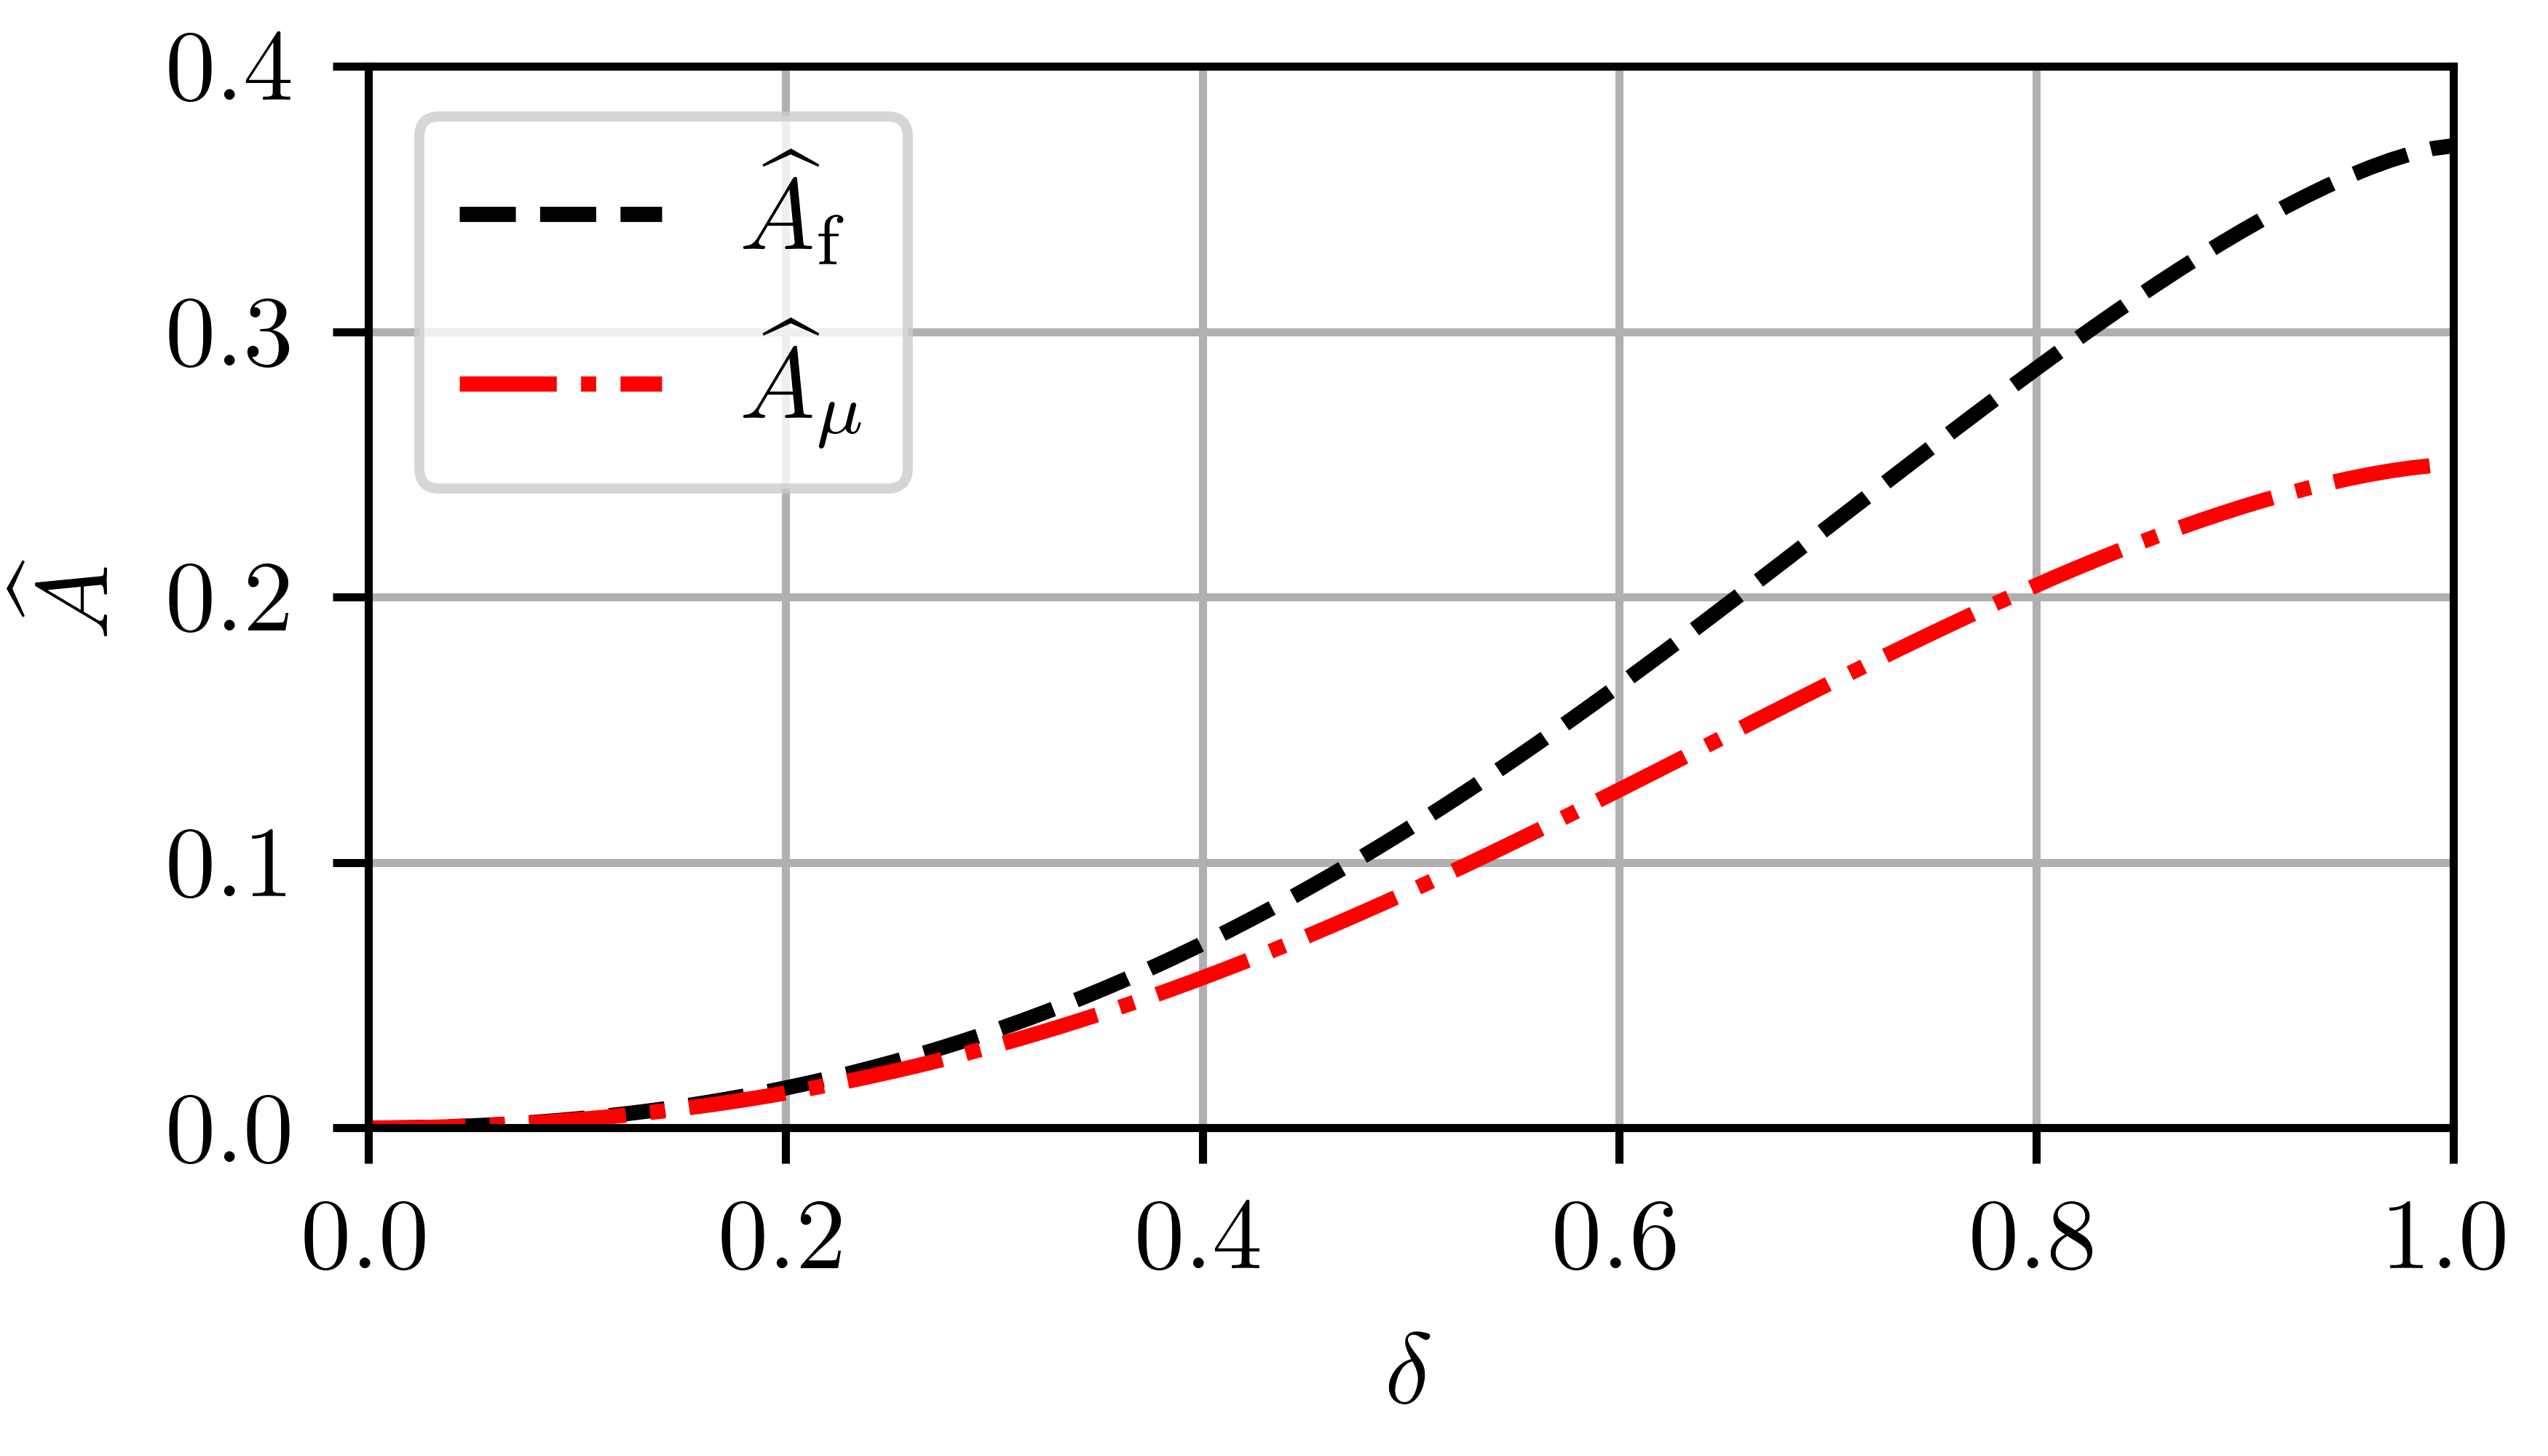
\includegraphics{3_chapters/0_introduction/img/AE.png}
    \caption{The \AE{} of the single waterbag distribution for both the case where there are no additional invariants, and $\mu$ is an invariant.}
    \label{fig: aes of the example}
\end{figure}
To gain some insight into the complex functional forms, let us consider two limiting cases. First, we Taylor expand around the smallness of $\delta$ to the third order, which results in $\widehat{A}_{\rm f}\approx \frac{5}{16} \delta^2 + \frac{5}{16} \delta^3$. Expanding the constrained case to the third order in $\delta$ also results in $\widehat{A}_\mu \approx \frac{5}{16} \delta^2 - \frac{1}{12}\delta^{5/2} + \frac{5}{16} \delta^3 $. We thus find that, to leading order, the contributions are exactly the same, and it is the leading order correction where differences in the behaviour of the \AE{} are found. The other limiting case is $\delta=1$ for which one finds $\widehat{A}_{\rm f}=1-2^{-2/3}$, and $\widehat{A}_\mu=1/4$. Therefore, we see that the \AE{} in the unconstrained case is, perhaps unsurprisingly, higher than that of the constrained case. Finally, a graph showing the full behaviour of the \AE{}s is given in Fig. \ref{fig: aes of the example}. In this Fig. we see that increasing the gradient (parameterised by $\delta$) increases the amount of available energy, given formal weight to the mantra that gradients supply free energy. \par

Let us now take a step back and investigate what we have learnt from the above example. In all cases, we have seen that we were able to derive the ground state by means of Eq. \eqref{eq: integral for ground state} or its equivalent form differential form \eqref{eq:integro-diff for ground state}.  This ground state was typically a state in which gradients are flattened as much as is possible under the given constraints. Finally, we have seen that the calculation of the ground state and its associated energy is typically the most involved step in the calculation of \AE{}.\footnote{We note that, under certain conditions, one may short-circuit these calculations by assuming that the initial distribution function is close to a ground state. An explicit expression of \AE{} may then be derived, without the need to calculate the ground state explicitly, and this work is currently in preparation with Helander. However, one of these conditions is broken in the case of trapped electrons \AE{} and results in flawed expressions, and as such we present the full calculation here.} These observations will remain true as we investigate more intricate cases, in which closed form analytical expressions of \AE{} are not available. If we impose that both $\mu$ and $\mathcal{J}$ be conserved, we will encounter exactly one such case.

\section{The \AE{} to be investigated}
As indicated in previous sections, this thesis focusses on the \AE{} of trapped electrons, in which Liouville's theorem, invariance of $\mu$, and constancy of $\mathcal{J}$ are enforced. This is not the first investigation of such a scenario, as specialised cases were already investigated by \citet{helander2017available,helander2020available}. In these papers, Helander investigates (among other things) under what conditions the \AE{} of trapped electrons vanishes and subsequently calculated the \AE{} in the specialised case of omnigenous systems. Focussing on the former (as the latter will be generalised further in the thesis), it was found that \AE{} vanishes if two conditions are met. First, the device needs to be exactly omnigenous, meaning that trapped particles do not drift radially outward, or in terms of Eq. \eqref{eq: dJdalpha} one needs $\partial_\alpha \mathcal{J} = 0$. Second, the bounce-averaged binormal drift (encapsulated by $\omega_\alpha$ as in Eq. \eqref{eq: omega_alpha}) needs to be faster than the drift wave. For a density gradient-driven drift wave, such conditions are met in maximum-$\mathcal{J}$ devices, further highlighting their stabilising properties. \par 

The remarkable feature of this conclusion (which can be derived by relatively simple means) is that it reproduces exactly the linear gyrokinetic instability thresholds which were derived by \citet{proll2012resilience} in 2012, showing that it is also a nonlinear threshold. This makes it an especially promising candidate for application to turbulence, as it coincides with known gyrokinetic results. The \AE{} may then be interpreted as a distance measure from the instability thresholds, quantifying how unstable a system is. \par 

This is not to say that the results cannot be generalised further, to account for ions, passing electrons, or even more exotic scenarios. An attempt at such a generalisation was made in \cite{helander2020available}, where ion species and passing electrons were accounted for as well, which in turn were coupled via quasineutrality. Let us note, though, that the result of such a calculation is {\it highly} dependent on the chosen invariants, and one may arrive at different conclusions by making different choices. One other such choice shall be considered at the end of the thesis as well for passing electrons, with implications on transport. 